\lecture{17}{3. November 2025}{Bending – Deformation of Beams}

\subsection{Bending Deformation of a Straight Member}
On \Cref{fig:f17_1}.a  square cross section of an undeformed member is shown. 
When a bending moment is applied it tends to distort these lines as shown on \Cref{fig:f17_1}.b.

\begin{figure} [ht]
  \centering
  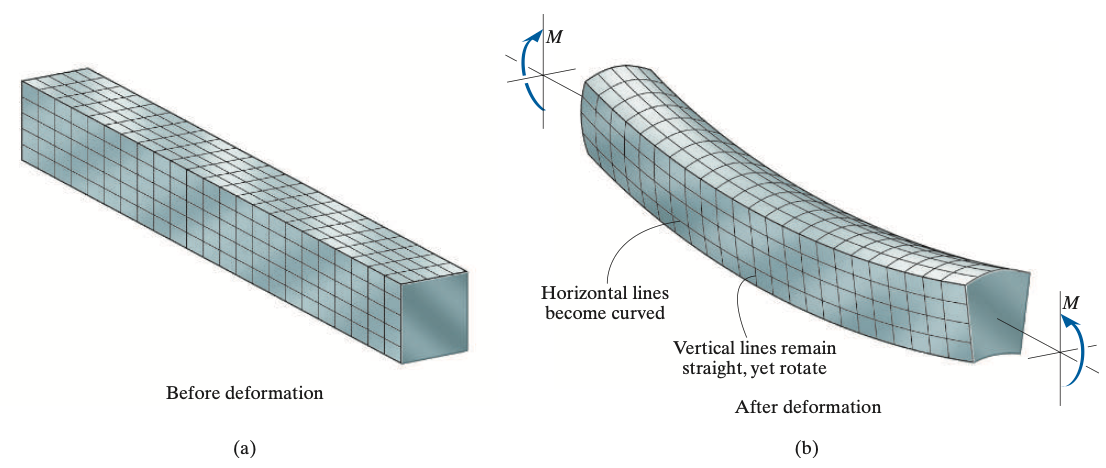
\includegraphics[width=0.8\linewidth]{./figures/f17_1.png}
  \caption{Bending deformation of a straight member.}
  \label{fig:f17_1}
\end{figure}

The horizontal lines become curved whilst the vertical lines remain straight but rotate.
A bending moment causes the material within the bottom of the member to stretch, whilst the top compresses.
Consequently, between these two regions there must be a surface called the \textit{neutral surface}, in which horizontal fibers of the material will not undergo a change in length.
As noted on \Cref{fig:f17_2} the axis that lies along the neutral surface is called the neutral axis

\begin{figure} [ht]
  \centering
  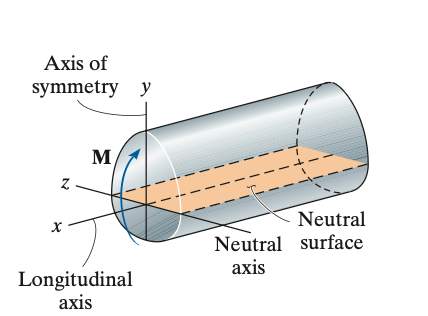
\includegraphics[width=0.35\linewidth]{./figures/f17_2.png}
  \caption{Neutral surface and neutral axis of a member.}
  \label{fig:f17_2}
\end{figure}

We now focus on the small member depicted on \Cref{fig:f17_3}.a located at a distance $x$ along the beam's length.
This element is shown in its deformed state on \Cref{fig:f17_3}.b.
Here, the line segment $\Delta x$, located on the neutral surface, does not change length, whereas any line segment $\Delta s$, located at an arbitrary distance above the neutral surface contracts and becomes $\Delta s'$ after the deformation.
The normal strain along $\Delta s$ is determined as
\[ 
\epsilon = \lim_{\Delta s \to 0} \frac{\Delta s' - \Delta s}{\Delta s}
.\]

\begin{figure} [ht]
  \centering
  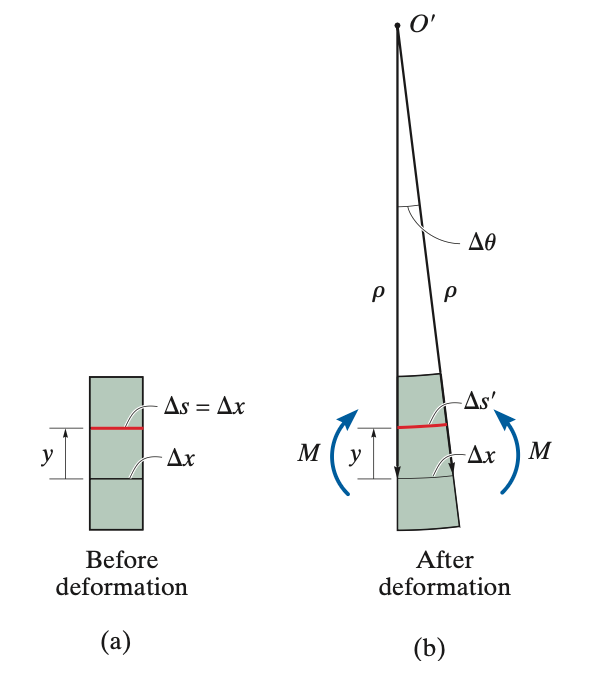
\includegraphics[width=0.5\linewidth]{./figures/f17_3.png}
  \caption{Bending moment on a small element}
  \label{fig:f17_3}
\end{figure}

We can also represent this strain in terms of the location $y$ of $\Delta s'$ and the radius of curvature $\rho$ of the longitudinal axis of the element.
We get:
\[ 
\epsilon = \lim_{\Delta \theta \to 0} \frac{\left( \rho - y \right) \Delta \theta - \rho \Delta \theta}{\rho \Delta \theta} = - \frac{y}{\rho}
.\]

Since $1 / \rho$ is constant at $x$ the above equation indicates that the longitudinal normal strain will vary linearly with $y$ measured from the neutral axis.
A contraction ($-\epsilon$) will occur in fibers located above the neutral axis ($+y$) and vice versa.
The maximum strain will occur at the outermost fiber, located at a distance of $y = c$ from the neutral axis.
Since $\epsilon_{\mathrm{max}} = c / \rho$ then
\[ 
\frac{\epsilon}{\epsilon_{\mathrm{max}}} = - \left( \frac{y / \rho}{c / \rho} \right)
\]
so that
\[ 
\epsilon = - \frac{y}{c} \epsilon_{\mathrm{max}}
.\]


\subsection{The Flexure Formula}
We consider a linear elastic material, meaning Hooke's law is applicable and results in a linear variation of normal strain.
Hence, the normal strain, $\sigma$ will vary from zero at the neutral axis to a maximum value $\sigma_{\mathrm{max}}$, a distance $c$ farthest from the neutral axis.
We get
\[ 
\sigma = - \frac{y}{c} \sigma_{\mathrm{max}}
.\]


\subsubsection{Location of the Neutral Axis}
To locate the position of the neutral axis, we require the resultant force produced by the stress distribution acting over the cross sectional area to be zero.
Based on \Cref{fig:f17_4}, we get
\begin{align*}
  F_R &= \sum F_x \\
  0 &= \int_{\mathrm{A}} \, \mathrm{d}F \\
  &= \int_{\mathrm{A}} \sigma \, \mathrm{d}A \\
  &= \int_{\mathrm{A}} - \frac{y}{c} \sigma_{\mathrm{max}} \, \mathrm{d}A \\
  &= - \frac{\sigma_{\mathrm{max}}}{c} \int_{\mathrm{A}} y \, \mathrm{d}A \\
  \implies \quad 0 &= \int_{A} y \, \mathrm{d}A
.\end{align*}
I.e. the ``first moment'' of the cross-sectional area about the neutral axis must be zero.
Therefore the neutral axis must also be the horizontal centroidal axis for the cross section.


\begin{figure} [ht]
  \centering
  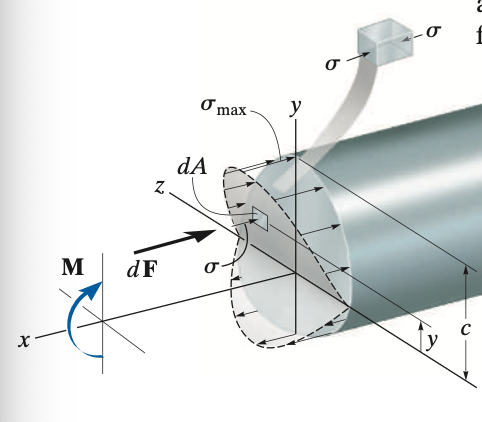
\includegraphics[width=0.4\linewidth]{./figures/f17_4.png}
  \caption{Bending stress variation}
  \label{fig:f17_4}
\end{figure}


\subsubsection{Bending Moment}
If we require the moment $M$ to be equal to the moment produced by the stress distribution over the neutral axis, the stress in the beam can be found.
I.e.:
\begin{align*}
  \left( M_R \right)_z &= \sum M_z \\
  M &= \int_{\mathrm{A}} y \, \mathrm{d}F \\
    &= \int_{\mathrm{A}} y \left( \sigma \, \mathrm{d}A \right) \\
    &= \int_{\mathrm{A}} y \frac{y}{c}\sigma_{\mathrm{max}} \, \mathrm{d}A \\
\implies \quad M &= \frac{\sigma_{\mathrm{max}}}{c} \int_{\mathrm{A}} y^2 \, \mathrm{d}A
.\end{align*}

This integral represents the \textit{moment of inertia} of the cross sectional area about the neutral axis.
Hence, symbolizing this as $I$ it can be rewritten as
\[ 
\sigma_{\mathrm{max}} = \frac{Mc}{I} \implies \sigma = - \frac{My}{I}
.\]

